\documentclass[a4paper,UKenglish,cleveref, autoref, thm-restate]{lipics-v2021}
%This is a template for producing LIPIcs articles. 
%See lipics-v2021-authors-guidelines.pdf for further information.
%for A4 paper format use option "a4paper", for US-letter use option "letterpaper"
%for british hyphenation rules use option "UKenglish", for american hyphenation rules use option "USenglish"
%for section-numbered lemmas etc., use "numberwithinsect"
%for enabling cleveref support, use "cleveref"
%for enabling autoref support, use "autoref"
%for anonymousing the authors (e.g. for double-blind review), add "anonymous"
%for enabling thm-restate support, use "thm-restate"
%for enabling a two-column layout for the author/affilation part (only applicable for > 6 authors), use "authorcolumns"
%for producing a PDF according the PDF/A standard, add "pdfa"

%\pdfoutput=1 %uncomment to ensure pdflatex processing (mandatatory e.g. to submit to arXiv)
%\hideLIPIcs  %uncomment to remove references to LIPIcs series (logo, DOI, ...), e.g. when preparing a pre-final version to be uploaded to arXiv or another public repository
\usepackage{graphicx}
\usepackage{amsmath, amssymb}
%\graphicspath{{./graphics/}}%helpful if your graphic files are in another directory

\bibliographystyle{plainurl}% the mandatory bibstyle

\title{Optimal Symmetry Breaking for Tournaments} 

%\titlerunning{Dummy short title} %TODO optional, please use if title is longer than one line

\author{Chris Lambert {Open Access}}{Dummy University Computing Laboratory, [optional: Address], Country \and My second affiliation, Country \and \url{http://www.myhomepage.edu} }{johnqpublic@dummyuni.org}{https://orcid.org/0000-0002-1825-0097}{(Optional) author-specific funding acknowledgements}%TODO mandatory, please use full name; only 1 author per \author macro; first two parameters are mandatory, other parameters can be empty. Please provide at least the name of the affiliation and the country. The full address is optional. Use additional curly braces to indicate the correct name splitting when the last name consists of multiple name parts.

\author{Evan Lohn\footnote{Optional footnote, e.g. to mark corresponding author}}{Department of Informatics, Dummy College, [optional: Address], Country}{joanrpublic@dummycollege.org}{[orcid]}{[funding]}

\author{Marijn Heule\footnote{Optional footnote, e.g. to mark corresponding author}}{Department of Informatics, Dummy College, [optional: Address], Country}{joanrpublic@dummycollege.org}{[orcid]}{[funding]}

\authorrunning{J. Open Access and J.\,R. Public} %TODO mandatory. First: Use abbreviated first/middle names. Second (only in severe cases): Use first author plus 'et al.'

\Copyright{Jane Open Access and Joan R. Public} %TODO mandatory, please use full first names. LIPIcs license is "CC-BY";  http://creativecommons.org/licenses/by/3.0/

\ccsdesc[100]{\textcolor{red}{Replace ccsdesc macro with valid one}} %TODO mandatory: Please choose ACM 2012 classifications from https://dl.acm.org/ccs/ccs_flat.cfm 

\keywords{Satisfiability,Symmetry-breaking,Directed-graphs} %TODO mandatory; please add comma-separated list of keywords

\category{} %optional, e.g. invited paper

\relatedversion{} %optional, e.g. full version hosted on arXiv, HAL, or other respository/website
%\relatedversiondetails[linktext={opt. text shown instead of the URL}, cite=DBLP:books/mk/GrayR93]{Classification (e.g. Full Version, Extended Version, Previous Version}{URL to related version} %linktext and cite are optional

%\supplement{}%optional, e.g. related research data, source code, ... hosted on a repository like zenodo, figshare, GitHub, ...
%\supplementdetails[linktext={opt. text shown instead of the URL}, cite=DBLP:books/mk/GrayR93, subcategory={Description, Subcategory}, swhid={Software Heritage Identifier}]{General Classification (e.g. Software, Dataset, Model, ...)}{URL to related version} %linktext, cite, and subcategory are optional

%\funding{(Optional) general funding statement \dots}%optional, to capture a funding statement, which applies to all authors. Please enter author specific funding statements as fifth argument of the \author macro.

\acknowledgements{I want to thank \dots}%optional
%\nolinenumbers %uncomment to disable line numbering



%Editor-only macros:: begin (do not touch as author)%%%%%%%%%%%%%%%%%%%%%%%%%%%%%%%%%%
\EventEditors{John Q. Open and Joan R. Access}
\EventNoEds{2}
\EventLongTitle{42nd Conference on Very Important Topics (CVIT 2016)}
\EventShortTitle{CVIT 2016}
\EventAcronym{CVIT}
\EventYear{2016}
\EventDate{December 24--27, 2016}
\EventLocation{Little Whinging, United Kingdom}
\EventLogo{}
\SeriesVolume{42}
\ArticleNo{23}
%%%%%%%%%%%%%%%%%%%%%%%%%%%%%%%%%%%%%%%%%%%%%%%%%%%%%%

\begin{document}

\maketitle

%
\begin{abstract}
In the field of satisfiability, symmetry breaking is a crucial technique needed to assist the solver in disregarding redundant candidate solutions.  As such, much work has gone into discovering `symmetry-breaking predicates' for common problems in satisfiability.  We extend prior work on undirected graphs to construct short, perfect symmetry breaking predicates on small tournaments.

\keywords{Satisfiability  \and Symmetry-breaking \and Directed-graphs}
\end{abstract}
%
%
% What is a tournament? What is an isolator? perfect isolator? optimal isolator? Why do we care?

% undirected graph isomorphisms
% https://math.stackexchange.com/questions/2725352/graph-combinatorics-upper-and-lower-bound-on-the-number-of-group-isomorphism-c

%nauty command: gentourng

%units
% no forced "at least one positive, negative"
%fewer isomorphism classes for small n
\section{Introduction}
Our main goal was to extend prior work \cite{ref_heule} with undirected graphs and generate optimal, perfect isolators for tournaments (complete, directed graphs). There were several places in which perfect isolator generation differed for tournaments.

\subsection{Global Clause Properties}
Because edgeless and complete graphs are isomorphism classes for any $n$ in the undirected case, every clause of an undirected graph isolator must contain at least one positive and one negative literal. These two graphs do not exist in the case of tournaments; the closest parallel is transitive tournaments satisfying $AB \land BC \rightarrow AC$ for every three vertices $A,B,C$ in the tournament. Unlike the undirected case (with exactly 1 empty graph and 1 complete graph), there are $n!$ isomorphic transitive tournaments on $n$ vertices. It is possible to select the particular transitive tournament $TT$ an isolator admits by ensuring that at least one edge from $TT$ is present in each clause of the isolator. A simple way to do so is ensure each clause contains at least one edge $AB$ s.t. $A<B$ in vertex numbering. However, this approach is not yet proven to admit an optimal isolator.

\subsection{Unit Clauses}
Another consequence of undirected isolators requiring at least one positive and one negative literal per clause is that undirected isolators have no unit clauses. However, tournament isolators have no such restriction and are thus allowed to have unit clauses. For $n<7$, the majority of clauses are unit in the optimal tournament isolators we present below.

\subsection{Ease of Isomorphism}
Another interesting difference between undirected graphs and tournaments is the low number isomorphism classes for tournaments when $n$ is small (see table \ref{tab:smallest_isolators_found}). Intuitively, this happens because it is ``easy'' for tournaments to be isomorphic. The two options for the edge between vertices $A$ and $B$ in the undirected case are $AB$ existing or not existing. Crucially, an undirected graph $G$ will never be isomorphic to $G'$ constructed by adding or removing an edge of $G$ (an operation that can be seen as ``flipping'' an edge to its other possibility). However, ``flipping'' an edge of a tournament $T$ (changing the edge's direction) will produce $T' \simeq T$ iff the two vertices $A$ and $B$ of the flipped edge had the same edges to the rest of the graph (the isomorphism is via the permutation that swaps $A$ and $B$).

\section{Methodology for Generating Isolators}

\subsection{Generation of Map Files}
Both of our approaches to generating isolators relied on the creation of ``map'' files: text files associating each graph of size $n$ with a label representing that graph's isomorphism class. In order to generate a map file for tournaments on $n$ vertices, we began by enumerating all $2^{n(n-1)/2}$ graphs of size $n$. We converted each graph into an adjacency matrix an then the ``.d6'' format specified in the NAUTY handbook, then fed the resulting graphs into the labelg script bundled with the NAUTY tool for graph isomorphisms \cite{ref_nauty}. labelg produced a file where each graph was converted to its canonical form. We gave each canonical form a unique label and output the arc (directed edge) indices of each original graph alongside its canonical form. Let $I_{ab}^n$ be the index of the arc from $a$ to $b$ in an $n$-vertex tournament.

The output format of the original graph arcs was extensible for higher $n$, satisfying the property that $I_{ab}^n = I_{ab}^{n+1}$. In particular, with $K = n(n-1)/2$ as the largest edge index for graphs of size $n$, the edges $(1,n+1), (2,n+1), ... (n, n+1)$ for $n+1$-vertex tournaments were labeled $K+1, K+2,...,K+n$, respectively. We will drop the superscript $n$ when referring to $I_{ab}^n$ in the future, as its value does not depend on $n$.

The arc indices described thus far only refer to the arcs in the direction of increasing vertex index, i.e. arc index 2 corresponds to $(1,3)$ and not $(3,1)$. We further define $I_{ab} = -I_{ba}$. However, when outputting graphs for the map file we simply exclude all negative arc indices to reduce file size, as the negative edges can be inferred with knowledge of $n$ because tournaments are complete graphs.

\subsection{Optimal, Perfect Isolator SAT encoding}

We re-implemented the basic structure of the perfect isolator encoding for undirected graphs \cite{ref_heule} with several modifications that mostly stem from the differences between undirected graphs and tournaments. The specific problem we encoded was ``Is there a set of $k$ non-unit clauses and a set of unit clauses whose union is a perfect isolator for $n$-vertex tournaments''. This first section will explain the encoding of the simpler problem: ``Is there a set of $k$ clauses whose union is a perfect isolator for $n$-vertex tournaments'', which will be modified to the final problem definition in following sections.

For each isolator clause $c$ and arc literal $a$, we defined the variable $In(c, a)$ to represent ``$a$ is in $c$''. Then, for each graph $G$ from the map file for $n$ vertices, we define a variable $Kills(G,c)$ to mean ``clause $c$ does not admit graph $G$''. This specification is implemented as follows with a Tseitin encoding \cite{ref_tseitin} to handle the equality:

\begin{equation}
Kills(G,c) = \bigvee\limits_{a \in A_G}In(c, a)
\end{equation}

where $A_G$ is the set of arc literals corresponding to the arcs present in graph $G$. We also define the variable $Canon(G)$ for all graphs $G$ from the map file, meaning ``Graph $G$ is the canonical representative of its isomorphism class.'' We implement this as follows (again using Tseitin to handle the equality and conjunctions):

\begin{equation}
    Canon(G) = \bigwedge\limits_c \lnot Kills(G,c)
\end{equation}

Finally, for each isomorphism class $E$ extracted from the mapfile as a set of graphs, let $E_1$ be the set ${Canon(G) | G \in E}$. We add the following clauses to the formula for each isomorphism class $E$:

\begin{equation}
 AMO(E_1) \land \bigvee\limits_{c \in E_1} c
\end{equation}
Where $AMO$ is the ``at most one'' operation on a set of clauses, implemented via a Sinz encoding \cite{ref_sinz}. In total, a satisfying assignment to this problem corresponds to a perfect isolator on $k$ non-unit clauses. If the problem is UNSAT for $k$ and SAT for $k+1$ non-units, this proves that the perfect isolator with $k+1$ non-units is optimal.


\subsection{Breaking Symmetries in the Encoding}

An easy symmetry in the encoding was the order of the isolator clauses.  Clearly, reordering clauses of an expression in CNF does not affect its behavior.  To resolve this, we added clauses that ensured a lexicographic ordering of the clauses in the resulting isolator.  For every adjacent pair of clauses $c_1$ and $c_2$, we fixed some ordering of every literal that may appear in them $a_1, a_2, \dots, a_n$, and then created variables $e_0, e_1, \dots, e_n$ where $e_i$ represents that clauses $c_1$ and $c_2$ are equivalent when considering only the first $i$ literals.  $e_0$ is always true, and to maintain the others we added the clauses
$$e_i = e_{i-1} \land (In(c_1, a_i) = In(c_2, a_i))$$
via the Tseitin transformation for every $1 \le i \le n$.  Then, we enforced a lexicographic ordering by requiring that for every $i$ such that $c_1$ and $c_2$ were equal up to $i$, that if clause $c_1$ contained $a_i$ then $c_2$ must also contain $a_i$.  Explicitly, we added the following requirement via the Tseitin transformation for every $1 \le i \le n$ and pair of adjacent clauses $c_1, c_2$
$$e_{i-1} \land In(c_1, a_i) \implies In(c_2, a_i)$$
and furthermore we required that $e_n$ is false to ensure a strict ordering.  When trying to find an isolator with $C$ clauses, this reduces the search space by a factor of $C!$ as only one permutation of a given set of clauses should be considered as opposed to all $C!$ of them.

We can find another symmetry in the ordering of the vertices.  We can reorder the vertices, and relabel the edge literals in an isolator accordingly, and this will result in another isolator that accepts the same graphs that the original did, but with the vertices permuted which keeps it in the same isomorphism class.  To break this, recall from the introduction that any tournament isolator must admit exactly one transitive tournament.  We may apply a permutation to this transitive graph (and the isolator) that turns it into a canonical transitive graph of $1 \to 2 \to 3 \to \dots \to n$.  Note that every edge in this graph goes from a lower numbered vertex to a higher numbered vertex, and so it would be a positive literal in our encoding and requires that this permuted isolator must have at least one positive literal in every clause.  As such, we know that for any isolator, there is a permuted isolator such that every clause has at least one positive literal in each clause.  We may add this to our encoding by requiring for all clauses $c$
$$\bigvee_{a \in A_p} In(c, a)$$
with $A_p$ being the set of all positive literals.    When trying to find an isolator for $n$ vertices, this reduces the search space by a factor of $n!$ since the solver is guaranteed to only consider isolators for which the canonical transitive graph is the $1 \to 2 \to \dots \to n$ described above.

\subsection{Encoding Unit Propagation}

Under the still rather naive encoding described above, the solver tended to find isolators where every clause was very large, but after applying unit propagation resulted in a much smaller, cleaner isolator that consisted of many units.  This indicated that not only was the solver generating solutions that needed postprocessing, but candidate isolators that were equivalent under unit propagation were being considered multiple times --- a sort of symmetry in this problem.  To resolve this, we added `unit clause' variables $Unit(a)$ representing ``literal $a$ is a unit clause''. We then required that the isolator be already unit-propagated with respect to the `unit clause' literals by adding the requirement
$$\lnot In(c, a) \lor \lnot Unit(a)$$
We also had to account for these units killing graphs in the $Canon$ clauses, so those were updated to be
$$Canon(G) = \bigwedge\limits_c \lnot Kills(G,c) \land \bigvee\limits_{a \in A_G}\lnot Unit(\lnot a)$$


Finally, we have to count these special unit literals towards the clause count in determining optimality.  However, in the practical sense units are essentially zero additional cost to an isolator: when used in a SAT solver they will be instantly eliminated through unit propagation and can only serve to reduce the complexity of the resulting problem.  From this line of reasoning, we might consider an `optimal isolator' to not just have the minimal number of clauses, but the minimal number of non-unit clauses.  Note that since units cannot exist in the undirected case, this alternative definition of optimality is consistent with the prior work on the undirected case.

We decided to not count units towards the clause count for use in determining optimality because of this.  This is not only a more useful definition, but results in a less complex encoding as we do not need to count objects of two different types, and we do not need to ensure that the non-unit clauses are actually not units.  The last is due to the fact that since units are `free' in our setup and non-units are costly, a solution to our encoding that uses a non-unit clause position to encode a unit will have wasted that position, and a solution that holds for fewer allowed non-units will simply move that clause to a unit literal position.

Note that using the direction symmetry breaking above, we only need to consider positive unit literals, which drastically reduces the search space in this step.

\subsection{Provable Units}

While constructing smaller isolators using the techniques above, we opted to manually inspect our results and see what patterns they shared.  Specifically, in the isolators up through 6 vertices there were some very noticable patterns in the unit clauses they contained, at least after permuting the isolators' vertices to line them up with each other.  The easiest structure to notice was that all of these isolators contained an $n-1$--length path, or a directed path that touches every vertex exactly once.  In graph theory literature, this is known as a Hamiltonian path.

As it turns out this pattern of units admits a proof, and so without worry we can include it in the basis for any isolator.

\begin{theorem}
All tournament graphs admit a Hamiltonian path.
\end{theorem}

\begin{proof}
Proceed by induction.  The statement is trivial for 1- and 2- vertex tournaments, since in the former the empty path is Hamiltonian and in the latter the sole edge is the path.  Now, given an $m$-length path in a tournament for $2 \le m < n-1$, argue that an $m+1$-length path exists.

Label the vertices on the given path by $1$ through $m+1$, and since $m+1 < n$ there exists some other vertex $a$.  If there is an edge from $a$ to $1$ or $m+1$ to $a$, then we can trivially extend the path to include $a$, so take the other case where there is an edge from $1$ to $a$ and an edge from $a$ to $m+1$.  Consider the smallest $1 \le i \le m+1$ such that there is an edge from $a$ to $i$.  Clearly $i > 1$ as there is an edge from $1$ to $a$, and clearly $i$ is well-defined since the set of $i$ where there is an edge from $a$ to $i$ is nonempty as it contains $m+1$.  Then, we have that $i-1 \ge 1$, and furthermore there is no edge from $a$ to $i-1$, so there is an edge from $i-1$ to $a$.  Therefore, we can take $i-2$ steps on the original path from vertex $1$ to vertex $i-1$, one step from $i-1$ to $a$, one step from $a$ to $i$, and $m+1-i$ steps on the original path from vertex $i$ to vertex $m+1$.  This new path has length $(i-2) + (1) + (1) + (m+1-i) = m+1$, completing the induction step and thus the proof.  $\square$
\end{proof}

It is worth noting that we do not have a proof that fixing a Hamiltonian path in an isolator is optimal.  However, getting a large set of units for free is extremely helpful, especially since our map-file approach does not need to consider graphs that are made impossible by a basis set of units. Including these units reduces the map file size and generation time by a factor of $2^{n-1}$, which makes map file-based approaches still viable for up to $n = 8$, and the risk of it being suboptimal (especially by a large factor) seems intuitively very low.


\subsection{Incremental Isolators}
One way to view the inclusion of a Hamiltonian path in our problem definition for each $n$ is that the unit clauses used to encode the isolator search problem for $n+1$ vertices build off the set of isolators used in the $n$ case (by simply adding the positive unit corresponding to the arc $(n, n+1)$). We further generalize this idea by showing that it is always possible to extend an isolator for $n$-vertex tournaments (and, incidentally, undirected graphs) to an isolator on $n+1$ vertices. Let $P_n$ be an isolator, defined here as a predicate on $n$-vertex tournaments that admits at least one tournament from each isomorphism class. Further, $[G]_n$ for a tournament $G$ on $n+1$ vertices refers to the tournament formed by removing the $n+1$th vertex of $G$.

\begin{theorem}
 For any $P_n$, a predicate $P_{n+1}$ that admits the $n+1$-vertex $G$ iff $P_n([G]_n)$ holds is an isolator on $n+1$-vertex tournaments.
\end{theorem}

\begin{proof}
Consider any canonical set containing representatives $R$ from each isomorphism class of $n+1$-vertex tournaments. For each $R$, $[R]_n$ is an $n$-vertex tournament and therefore a member of one of the isomorphism classes on $n$-vertex tournaments. By definition, the arbitrary given $P_n$ admits some $r$ such that $r \simeq [R]_n$. Any two isomorphic $n$-vertex tournaments are related by some vertex permutation $v_n$, where we define $v_n(r)$ for a tournament $r$ to be the tournament constructed by the application of $v_n$ to each vertex of $r$. Therefore we have $v_n(r) = [R]_n$ for some $v_n$.

This $v_n$ can be extended to tournaments on $n+1$ vertices via $v_{n+1}(x) = v_n(x)$ when vertex $x$ is not vertex $n+1$, and $v_{n+1}(x) = n+1$ otherwise.  Applying each $v_{n+1}^{-1}$ (the inverse permutation of $v_{n+1}$) to its corresponding $R$ yields a new canonical set $S$ for $n+1$-vertex tournaments because tournament isomorphism classes are closed under vertex permutation. We claim that $P_{n+1}$ admits all members of $S$, making it an isolator. To check this, note that each new canonical representative is of the form $v_{n+1}^{-1}(R)$ for some $R$. By definition of $P_{n+1}$, we must confirm that $P_n([v_{n+1}^{-1}(R)]_n)$ holds. However, $[v_{n+1}^{-1}(R)]_n = v_n^{-1}([R]_n) = r$, and $P_n(r)$ holds by the definition of $r$, completing the proof. $\square$
\end{proof}

The idea for incremental isolators and its following proof fell out of the observation that the optimal isolator for $n=5$ had striking similarities to the optimal isolator for $n=4$. In fact, it is possible to build directly off the entire $n=4$ isolator when constructing an optimal isolator for $n=5$. However, in general a perfect $n+1$-vertex isolator constructed incrementally from an optimal, perfect $n$-vertex isolator is not optimal, with a counterexample appearing at $n=6$. We note that it is also possible to build $n+1$-vertex incremental isolators from any subset of clauses from an $n$-vertex isolator. The most natural choice of subset when pursuing optimal isolators would be the unit clauses, because it kills the most non-canonical graphs. We were not able to prove that isolators built from incremental units are optimal or suboptimal in general, but it produces optimal isolators in practice up to $n=6$. The incremental units approach is a generalization to the approach of fixing the hamiltonian path units, and allows a further reduction of the space of considered isolators.

\subsection{Probing}
In addition to the SAT encoding approach to isolator generation, we also generated isolators using a method from prior work called ``random probes''  \cite{ref_heule}. On a high level, this approach starts with an empty set of clauses and adds randomly generated clauses that preserve at least one member of each equivalence class until the isolator is perfect.  There were only two non-superficial changes needed to adapt the prior work on random probes for undirected graphs to the directed case; allowing unit clauses and allowing clauses with only positive literals. While not guaranteed to generate optimal isolators, the strength of this approach is the relative speed with which isolators are generated. This approach also benefited in efficiency from the technique of disallowing clauses with all negative literals and extending isolators from the unit clauses of smaller isolators.

\subsection{nlogn proof}
%We seek to prove that at least $n\log{n}$???(placeholder) units can be part of an isolator for $n$-vertex tournaments.  
If a $TT_k$ is known to exist within every member of the class of $n$-vertex tournaments, each equivalence class must contain a member with the tournament fixed in some arbitrary position and orientation (i.e. vertices $1$ through $k$ in ascending order). Therefore, any isolator that fixes a $TT_k$ on the class of $n$-vertex tournaments is valid, i.e. will not remove any equivalence classes. Because the remaining subset of $n-k$ ``non-fixed" vertices also forms a tournament, further knowledge about the existence of a transitive tournament within the remaining $n-k$ vertices can be used to ``fix" (via units) another transitive tournament within the $n-k$ vertex subtournament. This procedure can be repeated until all vertices of the original tournament are part of some fixed transitive subtournament. Tournament Ramsey numbers provide exactly the required information about the existence of a transitive subtournament. Therefore, tournament Ramsey numbers can be used to construct sets of unit clauses for tournament isolators: we will refer to this as TT-fixing.

Let $units(n)$ be the function that returns the maximum possible number of units that can be added to an isolator when using the TT-fixing method on $n$-vertex tournaments. Our goal is to prove a lower bound on $units(n)$. Unfortunately, exact tournament Ramsey numbers are non-trivial to calculate (only up to $R(6) = 28$ is known). However, from Erd{\"o}s and Moser \textbf{CITE} we have that $R(k) \leq 2^{k-1}$, i.e. that a $TT_{k}$ must exist when considering any tournament on $2^{k-1}$ or more vertices. Erd{\"o}s and Moser's bound can thus be used with TT-fixing to lower-bound $units(n)$.


For a tournament on $n > 1$ vertices, we can express $n = 2^{k-1} + xk - c$ for some $x,k,c$ where $xk < 2^{k-1}$, $x>0$ and $0<c\leq k$. Intuitively, this rewrite makes explicit the largest power of 2 less than $n$ (calling that power $k-1$) and also makes explicit $x$, the number of times $k$ can be subtracted from $n$ before going below $2^{k-1}$. We note that each $TT_k$ fixed by TT-fixing corresponds to adding $\frac{1}{2}k(k-1)$ units, one for each edge in a $TT_k$. Also, the maximum number of units from TT-fixing is yielded by the greedy strategy of fixing the largest possible subtournaments first.

\begin{proof}
Assume for contradiction the existence of a class of tournaments that can be TT-fixed optimally without fixing the largest possible subtournament at each step. Consider in this TT-fixing result $F$ the first transitive subtournament $TT_s$ that is fixed with size $s$ and is smaller than $k$, the size of the largest possible subtournament that could have been fixed in $F$ at that step. Consider the partial result of TT-fixing up to but not including the insertion of $TT_s$ in $F$. At this step, continue a new TT-fixing $F'$ with a $TT_k$ instead of $TT_s$. Now, let $TT_s, TT_{s2}, TT_{s3},... TT_{sn}$ be the sequence of transitive tournaments fixed in $F$ defined by $TT_{sn}$ being the first fixed subtournament in $F$ for which the total fixed vertices up to and including $TT_{sn}$ reaches or exceeds the total vertices fixed so far in $F'$. All tournaments after $TT_s$ in $F$ must have $k$ or fewer vertices, because the maximum tournament size that can be fixed can never increase with any TT-fixing step and this size was $k$ when $TT_s$ was fixed. Therefore, $F$ up to $TT_{sn}$ exceeds the number of fixed vertices of $F'$ by at most $k-1$. \textbf{finish this? omit?}
\end{proof}


 Therefore $units(n) = units(2^{k-1} + xk - c) = \frac{1}{2}xk(k-1) + units(2^{k-1} - c)$.

We now seek to bound $units(2^{k-1} - c)$. $c \leq k$ and $units$ is monotonically non-decreasing (it is always possible to use at least the last fixing of transitive subtournaments via TT-fixing as $n$ increases), so $units(2^{k-1} - c) \geq units(2^{k-1} - k) $. Here we again rewrite the argument of $units$: $2^{k-1} - k = 2^{k-2} + x_1(k-1) - c_1$ with the analogous properties $x_1(k-1) < 2^{k-2}$, $x_1>0$ and $0<c_1\leq k-1$. We note that this rewriting procedure can be repeated until the introduction of $x_{k-1}$ \textbf{need to somehow mention this only works while $k>3$?}. In particular, 

\begin{equation}
2^{k-i} - (k - i) - 1= 2^{k-i-1} + x_i(k-i) - c_i  
\end{equation}


Analogously generalizing the number of units produced at ``step i'' (i.e. when the number of non-fixed vertices exceeds $2^{k-i-1}$) gives

\begin{equation}
units(2^{k-i-1} + x_i(k-i) - c_i) = \frac{1}{2}x_i(k-i)(k-i-1) + units(2^{k-i-1} - c_i)
\end{equation}
with proper restrictions on $x_i, c_i$. 

We can also use the equation that introduces $x_i$ to express it in terms of $i, c_i$ as follows: 

\begin{equation}
x_i = \frac{2^{k-i-1} + c_i - (k - i)}{k-i}
\end{equation}

Therefore, we express 
\begin{equation}
units(2^{k-1} - k) = \sum\limits_{i=1}^{k-1}\frac{1}{2}x_i(k-i)(k-i-1)
\end{equation}

Substituting $x_i$ and cleaning up the summation yields the following:

\begin{equation}
units(2^{k-1} - k) = \sum\limits_{i=1}^{k_1}\frac{1}{2}(2^{k_1-i} + c_i - (k_1 - i + 1))(k_1-i)
\end{equation}

where $k_1 = k - 1$. In general each $1\leq c_i\leq k - i$, and increasing $c_i$ increases $units(...)$, so we set $c_i = 1$ for the lower bound:

\begin{equation}
units(2^{k-1} - k) \geq \sum\limits_{i=1}^{k_1}\frac{1}{2}(2^{k_1-i} - (k_1 - i))(k_1-i)
\end{equation}

This summation can be split as follows:
\begin{equation}
units(2^{k-1} - k) \geq \frac{1}{2}\sum\limits_{i=1}^{k_1}(2^{k_1-i})(k_1-i) - \frac{1}{2}\sum\limits_{i=1}^{k_1}(k_1-i)^2
\end{equation}

And further rewritten for simplicity:

\begin{equation}
units(2^{k-1} - k) \geq \frac{1}{2}\sum\limits_{j=1}^{k-2}j(2^{j}) - \frac{1}{2}\sum\limits_{j=1}^{k-2}j^2
\end{equation}

At which point, it becomes clear that the sums have the following closed form:
% see https://math.stackexchange.com/questions/11464/how-to-compute-the-formula-sum-limits-r-1d-r-cdot-2r?noredirect=1&lq=1
% https://www.cuemath.com/algebra/sum-of-squares/
\begin{equation}
units(2^{k-1} - k) \geq (k-3)2^{k-2} + 1 - \frac{1}{12}(k-2)(k-1)(2k - 3)
\end{equation}

From here on out I use my highly suspect understanding of complexity theory...

Because we expressed $n = 2^{k-1} + xk + c$, we have $(k-3)2^{k-2} \in \Theta(n\log(n))$ and  $\frac{1}{12}(k-2)(k-1)(2k - 3) \in \Theta(\log(n)^3)$. Also, $units(n) \geq units(2^{k-1} - k)$ because $n \geq 2^{k-1} - k$. We conclude that an asymptotic lower bound on $units(n)$ is therefore $units(n) \in \Omega(n\log(n))$

\section{Results}

\subsection{Small Optimal Isolators}

Our SAT encoding allowed us to compute optimal isolators up to $n=6$. Figures \ref{fig1} and \ref{fig2} graphically display optimal, perfect isolators for $n=4,5$ by displaying a graph from each isomorphism class. Figure \ref{fig3} presents the same image for one of the 56 isomorphism classes for $n=6$. Most of the structure of these isolators can be seen from their unit clauses, which are depicted via red edges in the figures. For $n=4,5$ we also computed the number of different perfect optimal isolators up to isomorphism, where we define two isolators to be isomorphic if they are equivalent under some vertex permutation. There is only a single perfect optimal isolator for $n=4$, while there are 5 different (perfect optimal) isolators for $n=5$. Interestingly, each of the 5 can be expressed such that they have the same 6 unit clauses, and differ only in the 2 non-unit clauses present in optimal $n=5$ isolators.

\begin{figure}
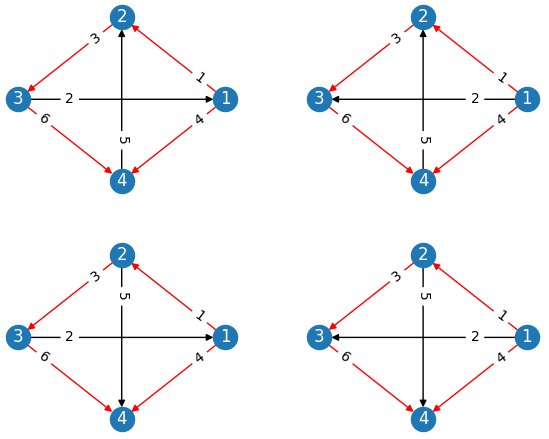
\includegraphics[width=0.6\textwidth]{iso_4.png}
\caption{Isomorphism class representatives admitted by a particular isolator for 4-vertex tournaments. Red edges are edges fixed by unit clauses of the isolator, and the isolator has only unit clauses.} \label{fig1}
\end{figure}

\begin{figure}
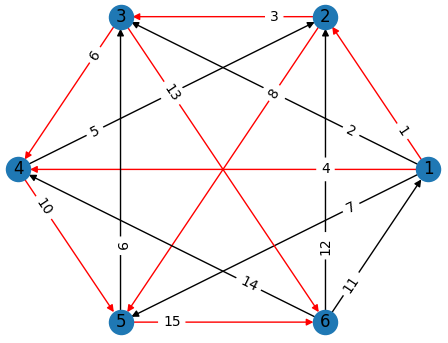
\includegraphics[width=0.4\textwidth]{iso6.png}
\caption{One of the 56 Isomorphism class representatives admitted by a particular isolator for 6-vertex tournaments. Red edges are edges fixed by unit clauses of the isolator.} \label{fig3}
\end{figure}
%mention the number of unique isolators up to isomorphism

\subsection{Larger Isolators}

In scaling up to larger graphs for isolators, we quickly run into barriers in our ability to solve problems in our encoding after $n = 6$.  For $n = 7$, solving the SAT instance directly became clearly infeasible (taking several days without any signs of progress). Random probing was the only method that allowed us to find an isolator; each probe ran in around 10 seconds when restricted to force a positive literal in each clause with the map file reduced by the unit clauses from $n=6$.  Table \ref{tab:smallest_isolators_found} describes the best isolator found during the semester for $n = 1$ through $7$. Several thousand probes were required to find our best known isolator for $n=7$.

\begin{table}[ht]
    \centering
    \begin{tabular}{c|c|c|c}
        Vertices &Best units & Best non-units & Isomorphism classes \\ \hline
        1&0&0&1\\ 
        2&1&0&1\\ 
        3&2&0&2\\ 
        4&4&0&4\\
        5&6&2&12\\ 
        6&8&6&56\\ 
        7&9&47&456\\ 
    \end{tabular}
    \caption{The smallest isolators found by number of non-unit clauses for all vertex counts up to 7, as well as the units in that isolator.  These are known optimal through 6 vertices.}
    \label{tab:smallest_isolators_found}
\end{table}

\begin{figure}
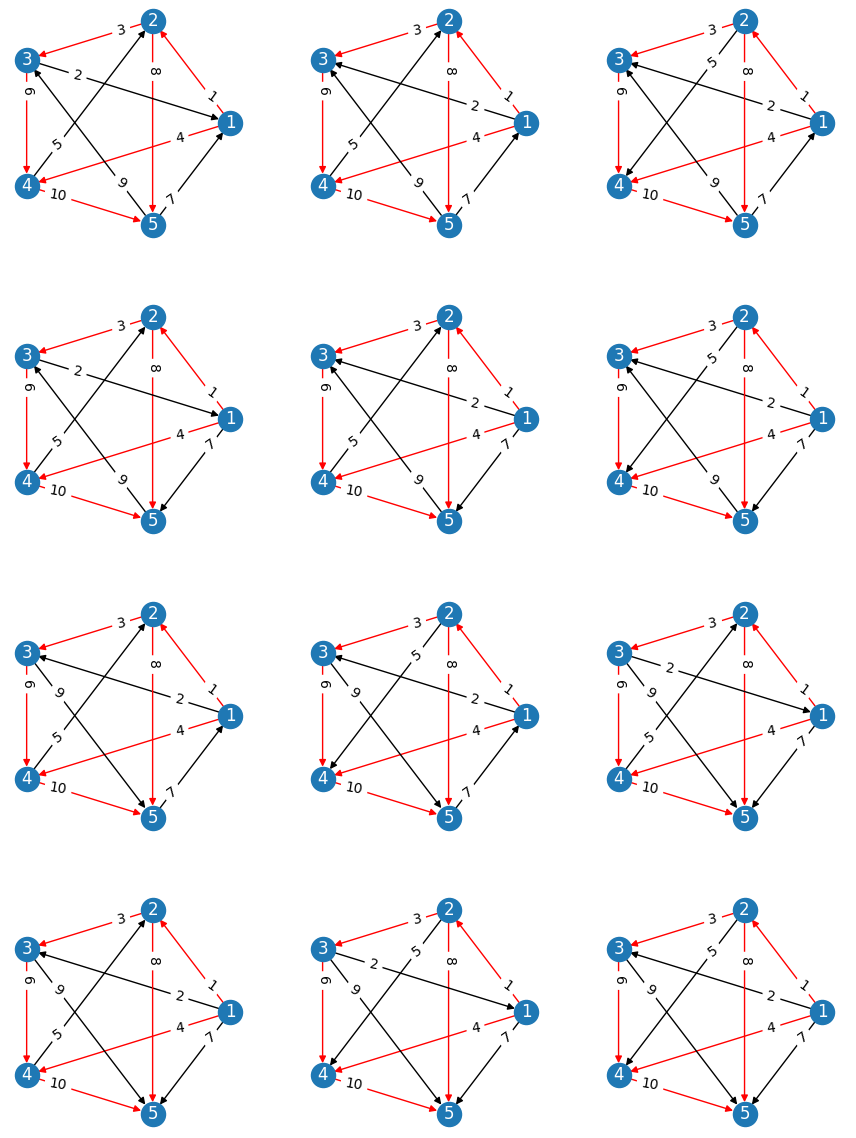
\includegraphics[width=0.9\textwidth]{iso_5.png}
\caption{Isomorphism class representatives admitted by a particular isolator for 5-vertex tournaments. Red edges are edges fixed by unit clauses of the isolator. The two non-unit clauses in the isolator are $2 \lor -5 \lor 9$ and $2 \lor 7 \lor -9$.} \label{fig2}
\end{figure}

%\subsection{Maximal Unit Sets}
%probably not needed, not actually interesting either without a bunch of figures to show the sets

\section{Future Work}

%\subsection{Limitations of Current Approach}

%imperfect but good isolators?
\subsection{Removing the Map File}

In our current setup, generation of the SAT problems involves mapping all possible tournament graphs to their isomorphism class.  Since this grows at a rate of $2^{O(n^2)}$, this becomes prohibitively large very quickly.  Even only considering graphs that satisfy a basis set of units, such as the Hamiltonian path or the prior isolator's units, these approaches quickly become infeasible as soon as $n = 9$.  By only generating the graphs that satisfy the previous isolator (and not just the units), this approach could potentially be extended for slightly longer, albeit at the cost of almost certainly suboptimal isolators.  A more clever encoding, or some way of encoding some of the ideas of graph isomorphism into the problem itself, could potentially drastically reduce the size of the problems and find isolators for much larger tournaments.

\subsection{Isolator Applications}

Graph existence problems, or problems that relate to whether a graph satisfying some conditions exist, are notoriously difficult to solve.  The Ramsey numbers, Conway's 99-graph problem, and many other problems can be phrased (or are most directly phrased) in this manner remain open problems in their fields even for relatively small instances.  For this reason computational approaches are tempting since they might be able resolve smaller instances of these problems, at least with an efficient enough algorithm.  Isolators provide a mechanism by which SAT solvers might be able to go fast enough to help in this area, since they drastically reduce the search space of possible graphs and leave only the non-redundant cases to check.

The main motivation towards finding these tournament graph isolators is their potential uses in computing tighter bounds on tournament Ramsey numbers --- the directed analog of Ramsey numbers for tournaments.  The tournament Ramsey number at $n$ is defined to be the smallest $m$ such that all tournaments on $m$ vertices contain a transitive (cycle-free) subtournament of $n$ vertices.  SAT approaches have been taken with this problem before to tighten bounds on the directed Ramsey number $R(7)$ \cite{directedramsey}.  From this it seems very likely that directed isolators --- boosted by their simplicity / number of unit clauses in them --- should be able to be applicable on this problem and potentially tighten those bounds further.


%\section{Generating Optimal Perfect Isolators}

%%Symmetry breaking is often a key challenge in encoding search problems into SAT instances. \textbf{mention some particularly important problems using SB}.

%The goal of graph existence problems is to prove the existence of an unlabeled graph satisfying certain conditions. For example, one method for computing Ramsey numbers (a foundational problem in Ramsey theory) is by showing that there exists a graph with $n$ vertices that contains a clique or independent set of size $k$, but there does not exist such a graph with $n+1$ vertices. 

%Graph existence problems can often easily be encoded to SAT by disallowing all sets of edges that could cause a graph to not satisfy the desired property (i.e. for Ramsey numbers, disallow all possible size-$k$ cliques and independent sets). However, the SAT approach to graph existence problems tends to be outperformed by specialized tools \textbf{CITE}. 

%The underperformance of SAT on these types of problems is at least partially due to suboptimal encodings \textbf{CITE}. We observe that if a graph $G$ satisfies $P(G)$, $G'$ satisfies $P(G')$ for any $G'$ constructed by permuting the vertices of $G$. With the naive problem encoding as input, a SAT solver may explore many symmetric parts of the search space that are all UNSAT. As such, it is often beneficial to augment problem encodings with a ``Symmetry-Breaking Predicate'' (SBP). In this work we generate compact symmetry-breaking predicates for small tournaments (complete, directed graphs) and prove several properties about their structure.

%The naive type of encoding mentioned above does not scale well as the number of vertices increases, as there are $2^{n(n-1)/2}$ possible graphs with $n$ vertices.

%\section{Background and Related Work}
%The work presented here can be seen as an extension of a similar paper generating optimal symmetry-breaking predicates for undirected graphs \textbf{CITE Optimal Symmetry Breaking for Graph Problems}.


\bibliography{main}

\end{document}
